\documentclass[conference]{IEEEtran}
\IEEEoverridecommandlockouts
% The preceding line is only needed to identify funding in the first footnote. If that is unneeded, please comment it out.
\usepackage{cite}
\usepackage{amsmath,amssymb,amsfonts}
\usepackage{graphicx}
\usepackage{textcomp}
\usepackage{xcolor}
\def\BibTeX{{\rm B\kern-.05em{\sc i\kern-.025em b}\kern-.08em
    T\kern-.1667em\lower.7ex\hbox{E}\kern-.125emX}}
\title{
\vspace{1cm}
{
\includegraphics[width=0.15\textwidth]{1.jpg} \\ 7474 Decade Counter} }
\author{Yalala Bhavani \\ Roll No: FWC22311 \\ bhavani27042003@gmail.com}
 \begin{document}
\maketitle
 \section {ABSTRACT}
 This paper shows how to use the 7474 D-Flip Flop ICs in a sequential circuit to realize a decade counter using arduino uno.

\section{COMPONENTS}
The required components list is given in Table: I., seven segment display is shown in Fig.1, IC 7447 diagram is shown in Fig.2 and 7474 D-Flip Flop pin diagram is shown in Fig-3.
\vspace{0.3cm}
 \begin{table} [htbp]
\centering
\begin{tabular}{| c | c | c |} \hline
Components & Value & Quantity \\\hline
IC & 7447 & 1 \\ \hline
IC & 7474 & 2 \\ \hline
seven segment display & & 1\\ \hline
Arduino & UNO & 1 \\ \hline
Jumper Wires &  & 50 \\ \hline
Breadboard & & 1 \\ 
\hline
\end{tabular}
\vspace{0.3cm}
\caption{\label{tab:widgets}}
\end{table}

\begin{figure}[h]                           
\centering                                 
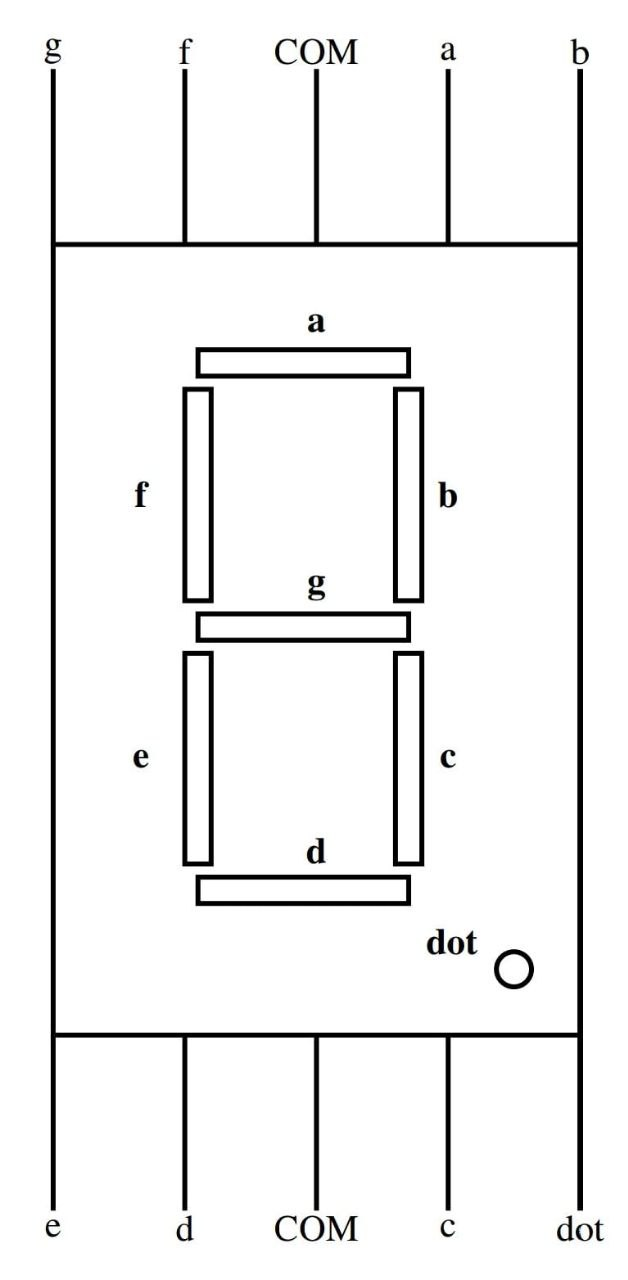
\includegraphics[width=0.2\textwidth]{ 2.jpg}                                           
\caption{\label{fig-1:Gates}}               
\end{figure}
\begin{figure}[h]                           
\centering                            
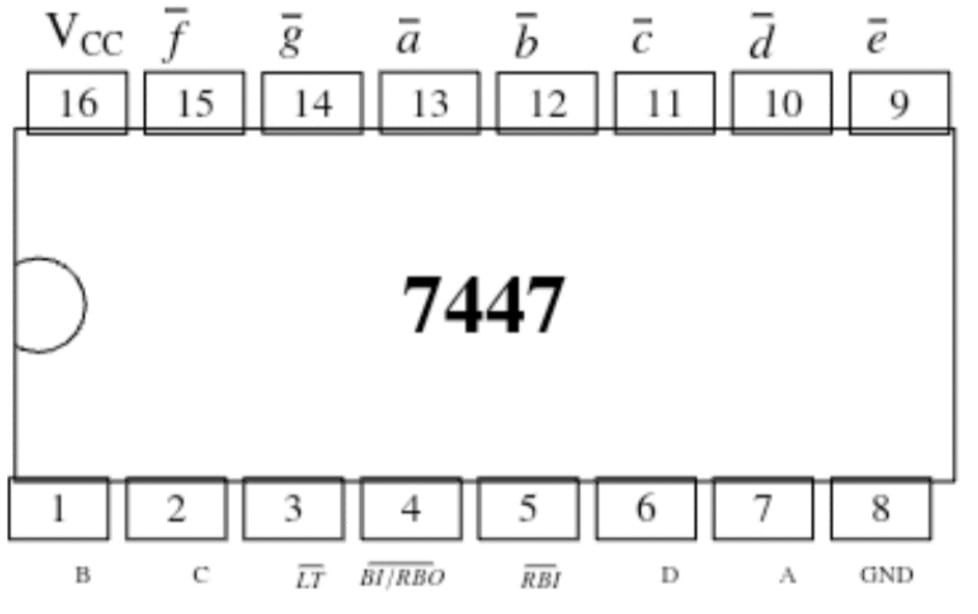
\includegraphics[width=0.5\textwidth]{3.jpg }                      
\caption{\label{fig-2:Gates}}           
\end{figure}

\begin{figure}[h]                           
\centering                                 
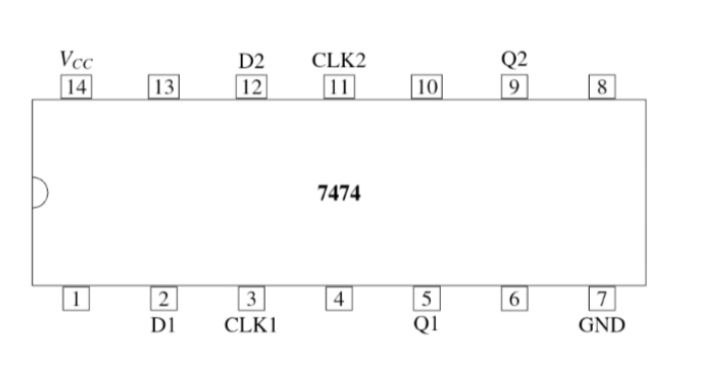
\includegraphics[width=0.4\textwidth]{ 4.jpg  }                                           
\caption{\label{fig-3:Gates}}               
\end{figure}

\section{PROCEDURE}


\begin{enumerate}

\item Make the connections of arduino, 7447 and two 7474 ICs according to Fig-4.
 \begin{figure}[h] 
 \centering 
 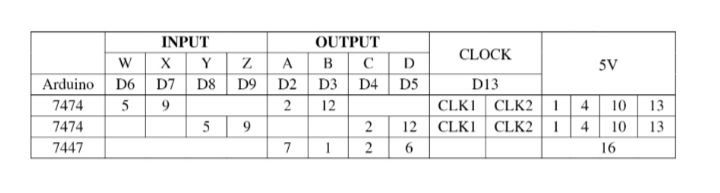
\includegraphics[width=0.5\textwidth]{5.jpg}
 \caption{\label{fig-4:Gates}}    
\end{figure}

\item Block diagram of Decade Counter.

\begin{figure}[h]                           
\centering                                 
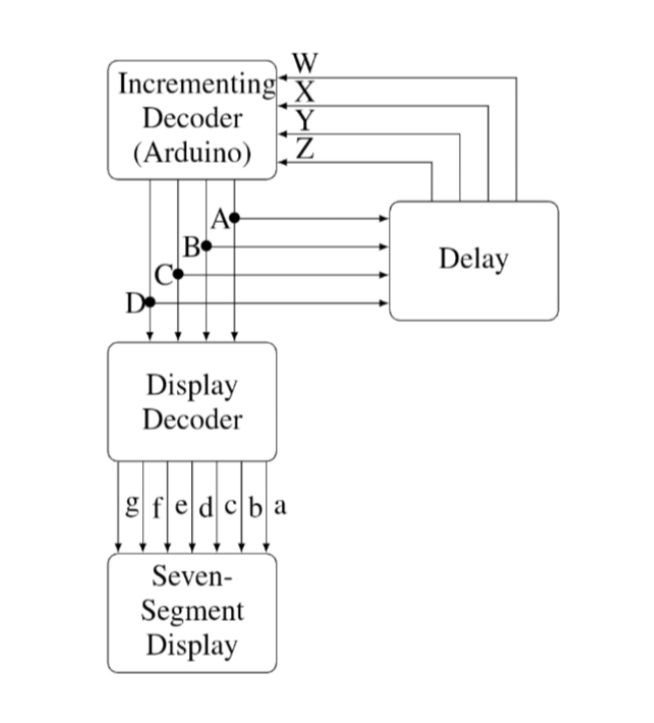
\includegraphics[width=0.3\textwidth]{6.jpg}                                           
\caption{\label{fig-5:Gates}}               
\end{figure}


 
\item Execute the arduino code without any errors.
\item After upload the code into hardware setup using arduino IDE platform with hex file.
 \end{enumerate}

\section{RESULTS}
 \begin{enumerate}
  \item Download the code given in the link below and execute them to see the output as shown in Fig.6. 
  \item https://github.com/Akhilathalla/Akhila/blob/main/7474/main.cpp
 \end{enumerate}
   \begin{figure}[h] 
 \centering 
 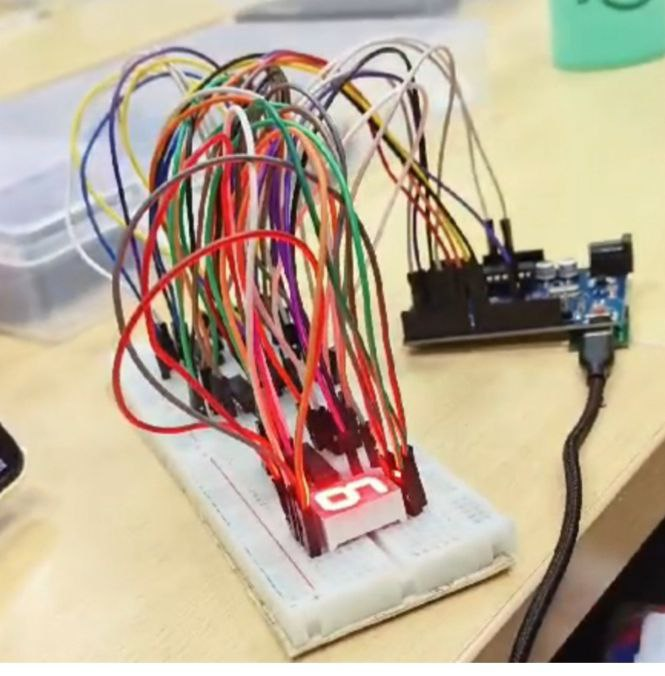
\includegraphics[width=0.4\textwidth]{7.jpg    }
 \caption{\label{fig-6:Gates}}    
\end{figure}
\section{CONCLUSION}
Hence implementation of 7474 IC Decade Counter on Seven segment dispaly using arduino UNO is done.
\end{document}
